\documentclass[12pt,a4paper,utf8x]{report}
\usepackage [frenchb]{babel}

\usepackage{graphicx}
\usepackage{caption}
\usepackage[utf8x]{inputenc}
\usepackage{multicol}
\usepackage{url} % Pour avoir de belles url
\usepackage {geometry}
\usepackage {listings} %Pour mettre du code source 
\usepackage{verbatim}
%\usepackage{lscape} % Pour pouvoir passer en paysage
\usepackage{colortbl}
\usepackage{xcolor}
\usepackage{textcomp}
\usepackage[strings]{underscore}

\geometry{left=2.5cm,right=2.5cm,vmargin=2cm}
\usepackage[pdftex,bookmarks = true,bookmarksnumbered = true,pdfpagemode = None,pdfstartview = FitH,pdfpagelayout = OneColumn,colorlinks=true,linkcolor=black,urlcolor=blue,citecolor=blue,pdfborder = {0 0 0}]{hyperref}


%chapitre---------------------------------------------------------------------
 
%%%% debut macro pour enlever le nom chapitre %%%%
\makeatletter
\def\@makechapterhead#1{%
  \vspace*{50\p@}%
  {\parindent \z@ \raggedright \normalfont
    \interlinepenalty\@M
    \ifnum \c@secnumdepth >\m@ne
        \Huge\bfseries {\color{black}\thechapter}\quad
    \fi
    \Huge \bfseries {\color{black}#1}\par\nobreak
    \vskip 40\p@
  }}

\def\@makeschapterhead#1{%
  \vspace*{50\p@}%
  {\parindent \z@ \raggedright
    \normalfont
    \interlinepenalty\@M
    \Huge \bfseries #1\par\nobreak
    \vskip 40\p@
  }}
\makeatother
%%%% fin macro %%%% 

\begin{document}

\begin{titlepage}
\begin{flushright}
   	
\includegraphics[scale=0.30]{univorleans.png}\\ 
   	   	Département Informatique
\end{flushright}
\vspace{30mm}
\begin{center}
\huge{Rapport de projet réseau}\\
\vspace{8mm}
\vspace{3mm}
\large{Proposé par : Sophie Robert}
\vspace{3mm}
\large{\\Réalisé par :}\\
\large{Fontorbe Jordan, Guillaume Arthur (Groupe: CJ)}\\
\end{center}
\begin{figure}[b!]
\begin{flushright}
~~\\ ~~\\ ~~\\ ~~\\ ~~\\ ~~\\ ~~\\
\large{Année universitaire: 2012-2013}
\end{flushright}
\end{figure}
\end{titlepage}

\tableofcontents
\clearpage

\chapter[Architecture des réseaux]{Présentation de l'architecture des réseaux}
Pour réaliser ce projet, nous disposions d'un réseau Netkit fournit avec le sujet.\\
Celui-ci se compose de plusieurs sous-réseaux:
\begin{description}
\item[hub]Le sous-réseau que nous avons dû configurer. Il est composé d'un routeur \emph{box} et de deux machines \emph{pc1} et \emph{pc2}. La configuration de ce sous-réseau que nous avons dû effectuer devait être faite uniquement à travers le routeur \emph{box}.
\item[rezo]Un sous-réseau extérieur à \emph{hub}. Celui-ci devait pouvoir communiquer avec \emph{hub}. Il n'était pas autorisé de modifier la configuration des machines de ce sous-réseau. Ce sous-réseau contient deux machines dont un serveur web.
\end{description}
\begin{center}
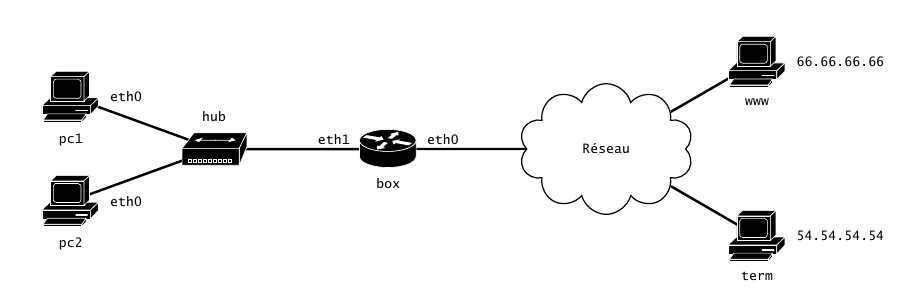
\includegraphics[width=1\textwidth]{archi.png}
\end{center}
\chapter{Travail effectué}
\section{Configuration du routeur}
Cette première partie consistait en la configuration du routeur \emph{box} pour que celui-ci puisse communiquer avec les réseaux extérieurs et avec les machines du sous-réseau \emph{hub}.\\
Pour cela nous avons éditer le fichier \emph{box.startup} comme suit:
\begin{verbatim}
ifconfig eth0 110.186.156.14
ifconfig eth1 10.176.63.1
route add default gw 110.0.0.1
\end{verbatim}
Les deux premières lignes servent à configurer statiquement les adresses IP des deux interfaces du routeur \emph{box}.\\
L'interface \textbf{eth1} est dans le sous-réseau \emph{hub} alors que \textbf{eth0} permet de communiquer avec le reste du monde.\\
La troisième ligne indique au routeur la passerelle par défaut qui permettra de communiquer avec les machines qui ne sont les sous-réseaux auxquels il appartient.
\section{Configuration du serveur DHCP}
Cette deuxième partie, a pour but de configurer un serveur DHCP sur le routeur \emph{box} afin d'attribuer des adresses IP de façon dynamique aux machines du réseau.
\label{lbl1}
\begin{verbatim}
default-lease-time 3600;
max-lease-time 86400;

subnet 10.176.63.0 netmask 255.255.255.224{
       range 10.176.63.3 10.176.63.30;
       option routers    10.176.63.1;
}
\end{verbatim}
Les deux premières lignes permettent de configurer les durées de validité des baux accordés par le serveur.
La valeur 3600 a été choisit arbitrairement. Elle est exprimée en secondes. Une durée de validité courte est privilégiée pour des sous-réseaux avec beaucoup de machines afin de pouvoir réutiliser les adresses rapidement après la déconnexion d'un client. A contrario une durée de validité plus longue sera privilégié pour réduire le trafic dans le sous-réseau.\\
Les trois lignes suivantes servent à attribuer dynamiquement une adresse IP comprise entre 10.176.63.3 et 10.176.63.30 sur le réseau privé 110.176.63.0/27 aux clients souhaitant rejoindre le réseau.
L'adresse 10.176.63.0 est celle du réseau et ne peut donc pas être attribuée à une machine. Tout comme 10.176.63.31 qui est l'adresse de broadcast de ce sous-réseau.\\
Enfin, l'adresse 10.176.63.2 est réservé pour une machine particulière du sous-réseau. Ceci sera détaillé dans le point 4 de ce chapitre (l'adresse 10.176.63.1 est utilisée par le routeur \emph{box}).
La dernière ligne sert à indiquer la passerelle par défaut aux machines se configurant via le serveur DHCP.

Voici un exemple des trames lors de le configuration par DHCP de \emph{pc2} :

\begin{figure}[h!]

	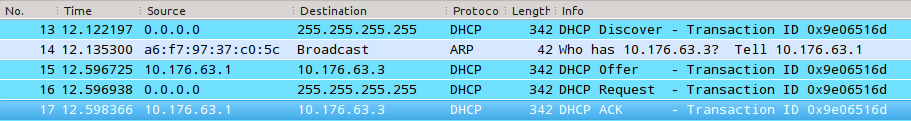
\includegraphics[width=1\textwidth]{TrameDHCP.png}
	\centering
	\caption{Trames de configuration par DHCP pour pc2.}

\end{figure}

\section[NAT dynamique]{Configuration de \emph{box} pour NAT dynamique}
Dans cette troisième partie, nous devions configurer le routeur \emph{box} pour faire du routage NAT dynamique. Cette configuration a permis aux machines du sous-réseau 110.176.63.0/27 de communiquer avec l'extérieur.
\\
\begin{verbatim}
echo 1 > /proc/sys/net/ipv4/ip_forward
iptables -t nat -A POSTROUTING -o eth0 -j SNAT --to-source 110.186.156.14
\end{verbatim}
La première ligne sert à activer sur le routeur \emph{box} "l'IP forwarding".
\\
La seconde ligne permet de remplacer, lors de la traversée du routeur par un paquet sortant l'adresse IP source par l'adresse IP extérieur du routeur afin de fournir au destinataire une adresse publique pour la réponse.
\\
Ci-dessous, des captures des trames sur les sous-réseaux \emph{hub} et \emph{rezo} de deux ping de \emph{pc2} vers \emph{term}:

\begin{figure}[h!]
\centering
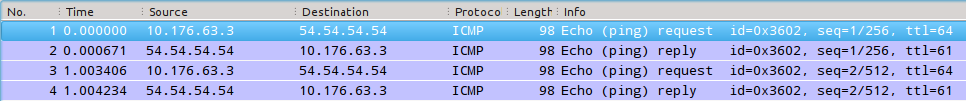
\includegraphics[width=1\textwidth]{PingHub.png}
\caption{Capture de trames lors d'un ping de \emph{pc2} vers \emph{term} sur \emph{hub}.}
\vspace{1cm}
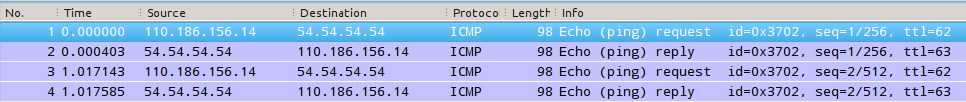
\includegraphics[width=1\textwidth]{PingRezo.png}
\caption{Capture de trames lors d'un ping de \emph{pc2} vers \emph{term} sur \emph{rezo}.}
\end{figure}

\section[Configuration statique de \emph{pc1}]{Attribution d'une IP statique à \emph{pc1}}
L'objectif de cette partie du projet était d'attribuer une adresse IP fixe à \emph{pc1}. Pour ensuite pouvoir rediriger sur \emph{pc1} les connexions SSH entrantes sur le routeur \emph{box}.\\
Les lignes suivantes ont été ajoutées au fichier dhcp.conf du routeur \emph{box}:
\begin{verbatim}
host pc1 {
	hardware ethernet 6e:5f:98:37:0c:07;
	fixed-address 10.176.63.2;
}
\end{verbatim}
Ce bloc indique au serveur DHCP que toute demande venant de l'interface ayant l'adresse MAC indiquée devra se voir attribuer l'adresse IP 10.176.63.2.\\
C'est pour cela que cette adresse n'appartient à la plage d'adresse attribuable par le serveur DHCP (voir \ref{lbl1} page \pageref{lbl1}).\\
Cette ligne a été ajoutée au fichier box.startup:
\begin{verbatim}
iptables -t nat -A PREROUTING -p tcp -i eth0 -d 110.186.156.14 --dport 22
         -j DNAT --to 10.176.63.2:22
\end{verbatim}
Celle-ci permet de rediriger tous les paquets TCP sur \emph{box} par l'interface \emph{eth0} vers le port 22 de \emph{pc1} (dont l'adresse IP viens d'être fixée).\\
Ci-dessous, une capture des trames sur le sous-réseau \emph{hub} lors d'une connexion SSH de \emph{term} vers \emph{pc1}, en utilisant l'IP publique de \emph{box}.
\begin{figure}[h!]
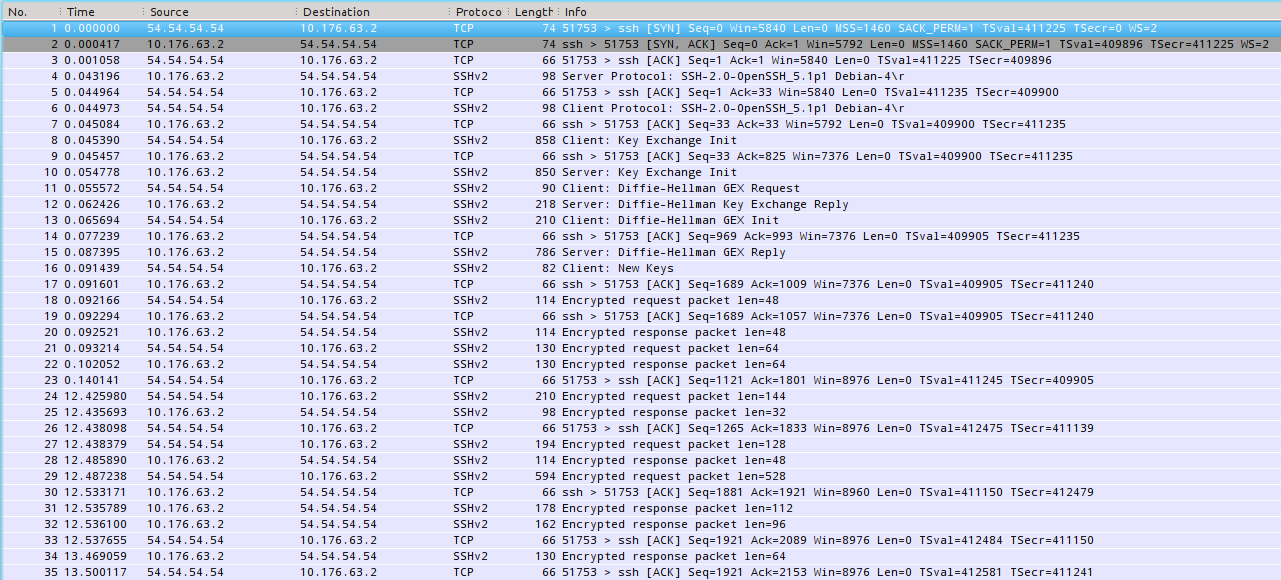
\includegraphics[width=1\textwidth]{SSHHub.png}
\caption{Capture de trames lors d'une connexion SSH de \emph{term} vers \emph{box} sur \emph{hub}.}
\end{figure}
\clearpage
\section[Filtrage sur \emph{box} des connexions entrantes]{Configuration de \emph{box} via IPTABLES pour un filtrage des connexions entrantes.}
Dans ce dernier point, il était demandé de détruire tout les paquets entrants sur \emph{box} à l'exception des connexions SSH depuis \emph{term}.\\
Pour cela, nous avons ajouté les lignes suivantes à box.startup:
\begin{verbatim}
iptables --flush
iptables -P INPUT ACCEPT
iptables -P FORWARD ACCEPT
iptables -P OUTPUT ACCEPT
iptables -A FORWARD -p tcp --syn -s ! 54.54.54.54 --dport ssh -j DROP
iptables -P INPUT DROP
iptables -A INPUT -i eth1 -j ACCEPT
\end{verbatim}
Les quatre premières lignes servent à réinitialiser les filtres d'IPTABLES.\\
La cinquième ligne, rejette tout les paquets qui ne proviennent pas de \emph{term} et qui sont redirigés par \emph{box}. L'option '--syn' autorise les paquets sortants.\\
L'avant dernière ligne permet de détruire tout les paquets avec comme destination \emph{box}.\\
La dernière ligne met une exception sur les paquets internes au sous-réseau \emph{hub}. C'est à dire, les paquets entrants sur le routeur \emph{box} par l'interface \emph{eth1} (dans le réseau \emph{hub}) ne sont pas détruits.\\
\end{document} 
